\chapter{Cross-Blockchain Protocol for Public Registries}

\begin{center}
{\large\uppercase{$\text{Oleksii Konashevych}^{[0000-0003-0068-5962]}$}} 

Erasmus Mundus Joint International Doctoral Fellow in Law,\\ Science and Technology. 

\vskip -6pt

\end{center}

\vskip 2cm




\vfill




\newpage

\begin{multicols}{2}

\section*{Abstract} 

This paper presents a concept of the protocol for public registries based on blockchain. The proposed mechanism allows creating a standard database over a bundle of distributed ledgers. It ensures a blockchain agnostic approach and utilizes the benefits of various blockchain technologies in one ecosystem. In this scheme, blockchains play the role of journal storages (immutable log), while the overlaid database is the indexed storage. The distinctive feature of such a system is that in blockchain, users can perform peer-to-peer transactions directly in the ledger using blockchain native mechanism of user access management with public-key cryptography (blockchain does not require to administrate its database). The protocol can be used to develop public property registries, i.e. land titles, cars, boats, corporate rights, etc. Users can create and manage their rights using the full power of blockchain technologies and smart contracts. The component of governance in this protocol is introduced as Smart Laws and Digital Authorities, the algorithms to manage the overlaid system and address legal issues with property rights and law enforcement.

\textbf{Keywords:} blockchain, electronic government, public registry, land registry, smart law, digital authority

\section{Introduction}
 
Governments play a crucial role in keeping public registries to prevent legal disputes about “who owns what.” Thus, the government acts as a trusted third party in private relations. However, if the government as a mediator loses the ability to be a source of law and order, it becomes a cause of conflicts.

Therefore, centralization, for instance, in state-owned land registry is a solution, but a source of risks. Risks are addressed by a system of hierarchically organized public administration, separation of powers, multiple checks and balances. It all becomes a burden for citizens that pay taxes and deal with red tape.

For a quiet time, it prevails Weber’s doctrine of the inevitability of bureaucracy \cite{art1-key01}. He believed that at this point of development, society should accept bureaucracy as inevitability and necessity.

The idea of the blockchain\footnote{The word “blockchain” is used here in the original meaning, i.e., a decentralized, uncensored public system. Hence, “permissioned” and “private” DLTs due to their centralized nature are not blockchains. Therefore, governments that use centralized technologies cannot claim the application of blockchain.} use for state-level governance and public registries is an open space for discussion in academia and blockchain industry, because it may reduce centralization.

A conceptualization in this field so far was limited to general ideas of “disrupting governance” (regulations, bureaucracy, middlemen, among others.) superficial in their essence, and unable answer how to design the system where law and technology will not collide exposing existing problems: enforceability in an immutable ledger of the blockchain technology, scalability, sustainable governance and many more discussed below.

Cross-Blockchain Protocol (CBP) is the technology of an overlaid database across a bundle of ledgers that enables smart laws and enforceability. The protocol is fundamental for the use of blockchains for property registries (for example, land cadastre) and other public databases run by governments. It may also have applications in the private and commercial sphere.

Alternatively, to an open and decentralized blockchain technology, tech consortia propose governments so-called “permissioned” (also known as private, federated, enterprise, etc.) Distributed Ledger Technologies (DLT), which are centralized, have similar vulnerabilities and limitations which other centralized technologies have. The advantages of such systems DLTs are questionable. There is no convincing evidence why this kind of technology is better than those centralized systems that governments have used for decades. It ensures immutability for records at the discretion of the authorities, i.e., retroactivity, censorship, corruption, and even full-stop of services are possible depending on a specific design of a system.

Moreover, DLTs have some unique features and some trade-offs, which may address one problem but will not be suitable for another. There is no reason to believe that any particular DLT is better than others and there will be one ultimate ledger. Hence, why would the government choose one DLT in favor to others?

But the major question in any technological shift is the cost of a mistake. Will governments have an opportunity to shift back or choose alternative technology with reasonable costs if anything goes wrong?

While one government agency runs one permissioned DLT solely, there is obviously no decentralization. If instead, a private network is in use, why would the government allow one private infrastructure provider (or a consortium) to monopolize the domain of public services?

Other questions may also arise. For example, if this is constitutional at all to share government sovereignty with a closed group of providers (nodes) that run a private network to provide public services? 

And finally, if a bunch of decent competitive and secure networks can provide reasonable infrastructure for public services, why choose one but not all?

Public blockchains, even though they are decentralized, it is not static.  Decentralization is ensured by constant fair competition. Bitcoin, Ethereum and some other public networks show that they remain sustainable. If some troubles happen on their ways, they still can tackle them without any central authority. Decentralization is the guarantee of the records to be safe and immutable. Centralized databases cannot provide such a level of immutability.

Therefore, this research is based on a hypothesis that public blockchains can be used as storage for records of land rights and other property rights (which normally are stored in government databases) and various government services, which also involves the need to store data in public databases.

Though immutability is not the only advantage. The traditional database cannot provide direct access for end-users; transactions are performed through registrars. Blockchains have a native mechanism to manage ownership with public key cryptography and the user can perform peer-to-peer transactions (title deeds). Thus, the user needs neither registrars nor registry keepers.

Once a token which represents the land title of the owner is created on the blockchain, there is no need to keep track of its transactions elsewhere. There is no need in any land registry because blockchain is the registry itself.

Nevertheless, people still need legal procedures, which now exists in paper form and applied by those registrars and other public bodies. Hence, the combination of blockchain and automation of procedures may significantly improve governance.

Such ideas remain for a while hypothetical, but this research is the first attempt to introduce a systematic approach of a system architecture for public services.

The proposed protocol aims to ensure that within the created bundle of existing blockchains, not the government, but citizens decide themselves where to keep their records of ownership and manage property rights. The bundle may unite not only public ledgers, but also permissioned, private, etc., and also interact with closed, centralized databases, which makes possible a shift from mono-database run by the government agency to multiple ledgers and cross-chain transfers.

This ensures fair competition among technologies, because users not only may choose any ledger within the bundle but transfer their assets from one chain to another if any technology does not suit their interests. On the other side, there is no need for the government to decide for citizens which technology to use, which corresponds with the principle of technological neutrality.

The protocol is a standard that transforms the “wild west” of incompatible and non-interactive networks into unified ecosystem. Notably, it does not require upgrades or permissions of these networks for the protocol to be applied.

Straightforward use of blockchain for running public registries is impossible. There are legal issues with enforceability and immutability, hardforks, digital identity, privacy, scalability and price volatility. The protocol is designed to address them.

It introduces the concept of “smart laws.” This is a framework for smart contracts and enforcement. Smart laws consist of algorithms that enable digital authorities to address legal issues: disputes, inheritance, loss of private keys, etc.

\section{Theoretical Framework, Methodology and Literature Review}
\subsection{Methodology and Theoretical Framework}

This paper is framed with design science research (DSR) provided by Hevner et al. \cite{art1-key02}. As per DSR, the research is meant to present an “artifact” which is defined as “constructs (vocabulary and symbols), models (abstractions and representations), methods (algorithms and practices), and instantiations (implemented and prototype systems).” This research deals mostly with \textit{models} and \textit{methods}.

In particular, the cross-blockchain database is a model, and cross-blockchain protocol is a set of methods of how this model can be designed. The research provides for a broad discussion and evaluation of the applicability of the proposed invention and constructs various models of its use in governance.

This research is complaint with 7-step research guidelines provided by Hevner et al., and corresponds with Design Science Research Publication Schema \cite{art1-key03} by Gregor and Hevner. The following table outlines steps of the performed SDR:

The following table outlines steps of the performed SDR: \textit{Method}. The primary method for this DSR is \textit{exaptation}, i.e., adoption of solutions from other fields. The research is looking into existing technologies which are applied here as elements of the protocol: Name-Value Storage, Berkley DB, RAID protocol, among others. The choice of Name-Value Storage as a reference technology for creating a database over blockchain is based on the analysis and comparison with two other similar technologies Bigchain and Amazon QLDB, presented in Section 4.1.a.
\end{multicols}
\begin{center}
\begin{tabular}{|l|l|m{13cm}|}
\hline
\textbf{\#} & \textbf{Step} & \textbf{Comment}\\\hline
1 & Introduction & Section 1 - the purpose and scope of the artifact – present a public registry model for property rights based on a bundle of existing public blockchains with enforcement and interoperability. Section 3 presents issues of the blockchain use by governments, which forms a corpus of research questions, which are to be addressed by this DSR.\\\hline
2 & Literature review & Subsection 2b provides context to the relevant academic research in blockchain and governance to support the integral elements of the protocol and proposed methods.\\\hline
3 & Method & Subsection 2a (this subsection)\\\hline
4 & Artifact description & Section 3 - a design concept of a cross-blockchain protocol for the creation of end-to-end public databases across a bundle of blockchains.\\\hline
5 & Evaluation & Subsection 4.3 is a technical evaluation of the architecture, its limitations and strategies to manage risks and constraints.\\\hline
6 & Discussion & Section 5 is a general evaluation of the technology applicability with legal and political aspects.\\\hline
7 & Conclusion & Section 6 is a summary of the research outcomes and discussion of further directions of the research.\\
\hline
\end{tabular}
\end{center}
\begin{multicols}{2}
The evaluation does not use experimental and testing methods for a few reasons. Firstly, there are no quantitative objectives (for example, there are no purposes to improve latency performance, bandwidth or size transaction optimization, among others); hence, there is nothing to measure for evaluation.

Secondly, the creation of a key-value DB across a bundle of public repositories is feasible enough to argue its implementation possibility.

The theoretical value of this research is more important since it meant to present viable models and scenarios of the use of decentralized blockchains, instead of permissioned DLTs in the public sector. The absence of any solution in this space practically makes the application of the public blockchain impossible, for instance, for property registries, due to known legal issues. Therefore, the hypothetical concept is valuable as it opens a discussion in the field.

Lastly, the development of the running system may require substantial resources. Therefore, broader independent evaluation and contribution among researchers many create more knowledge to consider development prototypes in the future.

Therefore, this research was focused on designing the concept of the protocol and, more generally, the concept of public registries across multiple blockchains, while all elements of this architecture exist and tested in various other applications.

\subsection{Literature review}

Recent academic literature creates a valuable context on the blockchain use, its benefits, applications, characteristics, classification and constraints.

The paper “Constraints and benefits of the blockchain use for real estate and property rights” \cite{art1-key04} became a basis for this research because it identified major constraints of the emerging technology for a public property registry, which laid down as the purpose to address in this research, i.e., to find the way to utilize benefits of blockchain for public property (real estate, land, etc.) registry and overcome major constraints (see Section 3).

A large portion of papers operate on a higher level when it comes to land registry, i.e., public services and e-government, seeking answers on how blockchain can improve this field. Among the first to discuss governance and blockchain was a journal paper “Beyond Bitcoin enabling smart government using blockchain technology” \cite{art1-key05} by Ølnes (2016). The author refers to the example of publishing hashes on Bitcoin - a small project at the University of Nicosia, where students were given electronic certificates after finishing a course, and a hash sum of the certificate was inserted in Bitcoin’s blockchain. Hashing on blockchain is much discussed in “Blockchain Anchoring of Public Registries: Options and Challenges” \cite{art1-key06}. The authors discussed  requirements for better system architecture for centralized public registry and DLT over it to hash DB entries.

In “Disrupting governance with blockchains and smart contracts,” \cite{art1-07} Shermin (2017) discusses the major constraints of the use of blockchain. There is a gap between the initial conceptualizations of blockchains and their first instantiations. First use cases show that as circumstances change, protocols can become inappropriate for the new environment and require modification. Modification of blockchain code happens through majority consensus, but reaching consensus in a distributed multi‐stakeholder network with sometimes unaligned interests is complex, potentially introducing new agency issues.

In “Blockchain technology as a support infrastructure in e-Government,” \cite{art1-08} Ølnes and Jansen (2017) continued the exploration of blockchain for governance. The authors are among the first to caution unreasonable optimism in the use of “permissioned” and “private” systems in public services: “Closed blockchains [...] must rely on traditional security mechanisms in order to prevent unwanted access and modification to the blockchain.” The paper mainly discusses open blockchains [networks], because as authors emphasize, “closed systems are never able to build an infrastructure.”

In “Blockchain in Government: Benefits and implications of distributed ledger technology for information sharing,” \cite{art1-key09} Ølnes, Ubacht and Janssen (2017) ask whether blockchain technology will lead to innovation and the transformation of governmental processes. To address this question, the authors presented a critical assessment of the “often exaggerated benefits of blockchain technology” found in the literature and discussed their implications for governmental organizations and processes. The paper summarizes directions for further research into the potential benefits of blockchain applications in e-government and the role of governance of blockchain architectures and applications to comply with societal needs and public values.

In “A framework of blockchain-based secure and privacy-preserving E‑government system,” \cite{art1-key10} Elisa et al. (2018) argue that most of the existing e‑government systems, such as websites and electronic identity management systems (eIDs) are centralized at duplicated servers and databases. A centralized management and validation system may suffer from a single point of failure and make the system a target to cyberattacks such as malware, denial of service attacks (DoS), and distributed denial of service attacks (DDoS). The blockchain technology enables the implementation of highly secure and privacy-preserving decentralized systems where transactions are not under the control of third-party organizations. They propose a framework of a decentralized e-government peer-to-peer system using blockchain technology to ensure information security and privacy while simultaneously increasing the trust of the public sectors. In addition, a prototype of the proposed system is presented with the support of a theoretical and qualitative analysis of the security and privacy implications of such a system. It is important to note that the authors share the idea that a “permissioned” (centralized) system can be called “blockchain.” They attribute this system features of blockchain: “The permissioned blockchain system ensures that the stored records are trustworthy, auditable and transparent.” In the proposed architecture, it is clear that infrastructure is introduced and maintained by the government. The question of how the proposed centralized system is better than the existing one remains open.

Batubara, Ubacht and Janssen published their “Challenges of blockchain technology adoption for e-government: A systematic literature review” \cite{art1-key11} in 2018. The paper guides through a number of studies and pilots in the use of blockchain in governance available by 2018. Several countries such as the USA, the United Kingdom, the Netherlands, the United Arab Emirates, Estonia, Sweden and China announced blockchain initiatives to explore its uses in the public sector actively. Their findings have shown that academic research in this area had only just started and issues discussed in the selected literature were still significantly limited. Consequently, more intensive research in this area was still necessary to advance this field's maturity. As per the authors, the major challenges from the organizational perspective are the need for new governance models and the acceptability of this technology. The research into blockchain technology standards and a reference architecture for e-Government applications was proposed to resolve the technological challenges.

Further directions are found in Franciscon et al. (2019) “A systematic literature review of blockchain architectures applied to public services” \cite{art1-key12}. This work provides a systematic review of blockchain-based applications across multiple domains: supply chain, business, healthcare, IoT, privacy, and data management. Authors point to the shortcomings identified in the relevant literature, particularly limitations the blockchain technology presents and how these limitations spawn across different sectors and industries. Building on these findings, authors identify various research gaps and future exploratory directions that are anticipated to be of significant value both for academics and practitioners.

 Brinkmann and Heine (2019) in “Can blockchain leverage for new public governance? A conceptual analysis on process level” \cite{art1-key13} presented the preliminary results of ongoing research, which aimed to shed light on the more concrete benefits of Blockchain for the purpose of New Public Governance (NPG). The preliminary results show that Blockchain offers valuable support for governments seeking methods to coordinate co-producing networks effectively. It becomes evident that there is a need for off-chain processes. Therefore, it is argued in favor of intensifying research on off-chain governance processes better to understand the implications for and influences on on-chain governance.
 
More recently, the paper “Smart Contracts for Government Processes: Case Study and Prototype Implementation” \cite{art1-key14} by Krogsbøll et al. (2020) contains a description of the pilot with the Danish Municipality. The government partner concluded that the risk of losing access to the system (due to loss of private keys) outweighed any benefits. The researchers on the other side think that smart contract implementations of government processes need to be immutable and outside of the government’s control when running; however, they also need to be updatable when laws change and provide an “out” for the rare case when errors in the contract implementation result in unlawful behavior and consider these problems as the “foundational research challenge for blockchain to be applicable to governmental processes.”

To sum up, the recent research introduced a variety of opinions about the blockchain technology, its features, benefits, and limits. This creates grounds for further research and development, especially application in various spheres of economic activity far beyond cryptocurrency. Yet to be noticed; still, a lot of perspective ideas remain in theoretical phases, or early stages of piloting. Therefore, the future challenge is to observe, collect and analyze more empirical data to define better practices and pitfalls across multiple fields and disciplines.

\section{Public blockchains issues}

This section defines problems on the way of the blockchain use for public registries: risks of multiplication of assets due to hardforks, enforceability, anonymity, digital identity, privacy, data integrity, scalability and price volatility. In the end, it is summarized what is opposed to blockchains and why blockchain is still a good choice for infrastructure.

\subsection{Why blockchain is impossible to use in public service as it is}

\subsubsection{Hardforks}

The hardfork is the major concern for systems with open competition because there are no authorities that impose and enforce one exclusive status quo. 

The system can split into two or more branches or so-called “forks,” after which each branch becomes independent but has a spare history of transactions till the moment of fork.

In the result of the split, tokens are duplicated. For example, if the system is used to manage rights on movable or immovable property (often mentioned as “asset-backed tokens”), in the result of a hardfork, the user will still have one plot of land but two title records in parallel systems. In the result of the fork, they can be managed independently, thereby creating legal collisions. For example, in one system, the user sells the plot, but in the other, the user still owns it.

\subsubsection{Immutability}

Being an advantage of blockchain technology, the immutability of the ledger can cause a lot of untoward use cases. For example, the loss of private keys will make cryptocurrency, a token, or a smart contract uncontrolled with negligible possibilities ever to restore it. Even if the blockchain can prevent many ownership disputes, the imperfect nature of people’s relationships will always cause issues with ownership and the need to settle when they arise. The blockchain itself, in its pure design, does not leave practical possibilities for enforcing any legitimate judicial decisions or any legal actions by authorities.

\subsubsection{Anonymity (pseudonymity)}

The authorization and authentication for a transaction are provided only with the relevant private key within the asymmetric pair owned by the user. The public key of the pair is taken to generate the address. The concept of addresses is the cornerstone of the blockchain. In the result of a transaction, a coin is spent from one address and added to another address, but to enable such transfer, the owner of the coin must use the relevant private key. Thus, the address is the only public record in the ledger that identifies the user. 

However, some research showed that addresses could be deanonymized by different digital fingerprints found in the network (IPs, behavior patterns, among others.) \cite{art1-key15}, \cite{art1-key16}. The pure blockchain protocol is not suitable for keeping records on property and securities from the perspective of governments — blockchain anonymity veils money laundering, financing terrorism, and other unlawful activity.

Beyond that, at the practical level, the censorless nature of the blockchain creates confusion in identifying records. Anyone may perform any transaction and publish any data in the blockchain. If the government must authorize a land title deed, how do you define if any transaction on the blockchain belongs to the town clerk if they are all pseudonymous? Without overlaid solutions for digital identities and trust services, it is almost impossible to create any scalable model for governance.

\subsubsection{Data integrity, off-chain data and issues of personal data}

In blockchain, any published data is exposed, and removal is not an option. Alternatively, users can insert into the blockchain cryptographic hashes of the data. The blockchain that stores hash sums will provide for two things: the user can verify the authenticity of the data (whether it is still the same or not) and timestamping because blocks are chronologically stored.

However, hashing does not ensure the protection of the data itself. Once it is tampered with and/or deleted, the hash sum is useless for restoring. This leads to two possible solutions: data will be stored by the third party (for instance, a government agency) or users themselves.

Today all personal data and property records (title records) are stored in closed databases controlled by governments, and publishing hashes whether into the centralized DLT or open blockchain does not add much security. To verify this data, the user needs access to that closed database or just blindly trusts the entity which stores it.

Even if public blockchain is used to store hashes, there is still in this scheme a trusted party as the source of “truth,” and so concentrating many risks for leaks and corruption of data as a single point of failure.

\subsubsection{Scalability}

One exclusively chosen blockchain for governance will necessarily create issues. Again because of the open and free nature, the blockchain protocol does not restrain publishing junk data in the ledger.

The potential bandwidth of Bitcoin per year, for example, is roughly 220 million transactions \cite{art1-key17}. For instance, 300 public registries in Ukraine generate as much as Bitcoin’s bandwidth \cite{art1-key18}, which leaves no space for other cryptocurrency transfers.

Overload with the transactions creates the problem of high transaction fees and price volatility. Although Bitcoin is not the best in terms of bandwidth, it is still the most attractive in terms of security \cite{art1-key19}. This is not a workable solution on a scale, even for one country with a 40-mln population, randomly chosen as an example.

For blockchain using other consensus protocols or other data structure, scalability is not the main issue. For example, Ethereum, IOTA, NXT, NEM, and many other systems ensure better bandwidth and performance.

The choice of one network in favor of others is a discussion about technological neutrality – a principle that is often discussed in the context of public policy. The reader may find discussions that compare one specific blockchain network with some specific centralized system, where usually blockchain performance is fewer. Having in mind the principle of technological neutrality, it is proposed to consider the problem of scalability from another perspective. One blockchain network does not necessarily provide enough scalability, while a bundle of blockchains may become much more effective.

\subsubsection{Price volatility}

Due to speculations, the price can dramatically fluctuate; therefore, creating a bad user experience for those who need cryptocurrency to pay fees for publishing and managing data and running smart contracts. Together with the mentioned scalability issues, it makes it infeasible for the government to use or even to announce their intention to use any specific blockchain. It will inevitably incentivize agiotage on the market, exacerbating the problem of scalability even more.

\subsection{What is opposed to blockchains and why it is still a good idea to use them}

Eventually, as might be thought, the permissioned DLT is much better than the blockchain, as it addresses all these issues due to its centralized nature, purposed to control and restrict unwanted practices and manually fix troubles.

There is no one specific consensus for permissioned systems. This is rather a title of various design concepts aimed to leave the leverage of control over the network in the hands of an authority, which can be by one actor or a closed group of actors.

Some protocols were not initially developed for permissioned design. For example, the Proof-of-Stake protocol (PoS) \cite{art1-key20} is designed as a cheaper alternative of Proof-of-Work. In PoS, network if a node (or a group of nodes who mutually agreed) has enough stake at their control, they may perform retroactive actions by rolling back blocks \cite{art1-key21} and can censor transactions.

Proof-of-Authority \cite{art1-key22}, and a family of Hyperledger consensuses \cite{art1-key23} protocols are dedicated to architecture with controlling features.

It is possible to design different schemas with privileged (“master”) nodes that are authorized for the creation of blocks, writing transactions, and some other specific rights providing those other participants of the network will not have them. Such systems can also be closed; therefore, users will need the authorization to read the information from blocks, whereas some protocol provides anonymous interaction (see, for example, DLT Quorum \cite{art1-key24}). Compared to existing centralized closed government systems, such DLTs may have some advantages; however, conceptually, they are the same. They are centralized and censorable and are not necessarily immutable for those who control it.

Another reason why the choice of one DLT leads to centralization is that the choice of one exclusive network prevents competition. By choosing a permissioned DLT, the government takes responsibility for developing and maintaining infrastructure.

On the contrary, open blockchain systems do not have central authorities that build the network. Any user is free to add their computational resources for public needs and therefore, compete for having rewards for finding blocks, and this reward is not distributed by someone centrally but automatically obtained as per the protocol. The infrastructure is self-organized incentivized by cryptocurrency with free competition for mining, i.e., creating and storing blocks.

The principle of decentralization is the basis of this research; therefore, we neither argue nor compare blockchain to centralized solutions. Centralized databases have already been in use for quite a long time by governments; therefore, we already know their advantages and disadvantages. Therefore, permissioned systems cannot be considered a significant evolutionary step in government systems.

Blockchain is a new word in governance, but this technology has some principal features that can restrain its implementation at the state level, and the following research conceptualizes ideas to address them.

Among various properties of the blockchain technology, we distinguish the following highly considerable for a new generation of public property registries:
\begin{itemize}
\item[-] Blockchain provides an append-only type of database, which is called an immutable ledger. It prevents data corruption and unauthorized changes.
\item[-] Blockchain has a native mechanism for managing ownership through public-key cryptography; thus, it is not only an immutable storage, but also it is a system for peer-to-peer transactions. On the contrary to traditional, for example, real estate registry, it does not require a trusted third party to record a deed in the database.
\item[-] Blockchain is self-organized and does not require central authorities to govern and maintain the infrastructure.
\end{itemize}

The proposal in this research concept utilizes the immutability of the blockchain with the help of “smart laws.” It reduces centralization when possible and makes it accountable when centralization is inevitable.

\section{Building a database across blockchains}\label{sec-4}

The first subsection introduces an idealistic design model of a database across a bundle of blockchains (Subsection~\ref{subsec-4.1}). Subsections~\ref{subsec-4.2} and \ref{subsec-4.3} analyze constraints of the model and evaluate possible design solutions to get the system working.

\subsection{General idea and basic elements}\label{subsec-4.1}

\subsubsection{General idea}\label{subsubsec-4.1.1}

A cross-blockchain database is a logic superstructure over a bundle of blockchains, see Fig~\ref{chap1-fig01}. To create a mutual interaction, users should agree which blockchains they include in the bundle and according to which rules and filters - the cross-blockchain protocol - they create the database.

The designed system collects users’ records from the blockchains of the bundle into a consistent end-to-end public database. The “record” is an entry the user inserts into any blockchain in the bundle, it can be a token (or a “colored coin”) or a key-value record.

An entry must be compliant with the format so the algorithm will automatically select and send in into the cross-blockchain database from heterogeneous data flow in blockchains (take into account that blockchain is uncensored; therefore, a lot of chunk data is also published there). This is the role of the protocol. It scans upcoming blocks in every ledger of the bundle and searches for records of a specific standard. 

It verifies each record as per the rules provided by the protocol and filters out if a record is non-complaint. Eventually, the system inserts the complaint record into the database, which is a local file on the user’s computer.

When a user applies the same protocol on any computer, he or she will receive the same copy of the database that every other user has on their local computers. Thus, there is no mathematical consensus for the database itself. The database relies on existing consensus protocols of those ledgers, which are included in the bundle. 

The consensus of the overlaid structure is a sort of a social contract because users must agree on the initial architecture of any particular database: which ledgers to scan and from which blocks, the format of the entry, and filtering rules, how to add new ledgers and drop a ledger from the bundle, how to transfer entries from ledger to ledger, how to upgrade and create patches in the protocol by collective decisions or by a central authority, etc. Thus, by applying the protocol and scanning blocks, users independently build a copy of the database.

%~ \begin{figure}[H]
%~ \centering
%~ 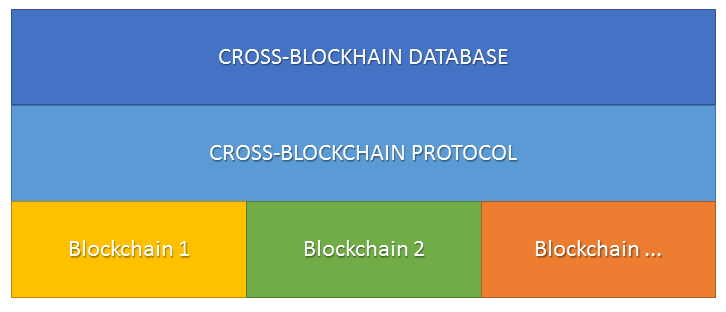
\includegraphics[scale=.85]{src/Figures/chap1/chap1-fig01.jpg}
%~ \caption{Basic scheme of a bundle of blockchains with overlaid database}\label{chap1-fig01}
%~ \end{figure}

\begin{quote}
The bundle can contain any number of ledgers but at any point in time, the list must be definite. The protocol provides for format rules and filters for entries and rules for scanning, adding new and deleting included ledgers intro the bundle. The system scans block across ledger of the bundle and hooks records that are compliant with the rules and adds them to the database.
\end{quote}

The blockchain provides for a native mechanism of ownership through public-key cryptography: the user publishes a record and the protocol considers the address from which he or she created this transaction as the owner of the record. Thus, to perform any update, the user must create a new record using the same private key because the private key is the authorizing mechanism for the address.

This mechanism was developed by a number of blockchain projects. To better explain this protocol, let us refer to Emercoin’s Name-Value Storage (NVS) technology, which is working since 2014 as one of the successful designs for storing arbitrary users’ data in the structured form in the database. Emercoin’s itself became a successor of a Namecoin’s non-ICANN TLD service (Top-Level Domain “.bit”). 

It should be noted that other types of databases and technologies may be applied, and therefore, it will require a compatible format of a DB entry.

Emercoin’s NVS protocol details are specified in Annex. We can extract a set of useful elements of both Emercoin’s and Namecoin’s NVSs. The following subsection presents which elements should be taken as a basis for a cross-blockchain protocol.

To address the legitimate question of why other types of blockchain-enabled databases, for instance, Bigchain and Amazon QLBD, were not chosen as a reference technology, it is considered the following. Bigchain is a framework that connects DLT framework Tendermint and MongoDB \cite{art1-key25}. The first version of the technology appeared in 2015, a year later then Namecoin and Emercoin. Amazon QLDB is a similar concept that connects the Hyperledger and PartiQL database \cite{art1-key26}, created in 2019. Both projects have one common feature, i.e. they took one of the existing DLT frameworks (Tendermint and Hyperledger Fabric) and use them as log systems for databases (MongoDB and PartiQL). DB entries are inserted in ledger transactions, then hooked and pushed through to the connected database. As we see, similar happens with Namecoin and Emercoin. Though, the difference is that public blockchain due to having native tokens (cryptocurrency) have embed user access mechanism through public key-cryptography, where a user’s address is a representation of a public key, and a private key is used to authorize transactions by digital signatures. The database entry to get through the blockchain is wrapped in a coin-spending transaction; therefore, they use their native mechanism of access management and authentication. Each DB entry is natively attached to the address to which it has been published.

In stacks like Bigchain\footnote{Note, that is coin-less DLTs “transaction” is an arbitrary byte array, see for reference Tendermint specification \url{https://github.com/tendermint/spec/blob/953523c3cb99fdb8c8f7a2d21e3a99094279e9de/spec/blockchain/blockchain.md}} and Amazon QLDB\footnote{In the block example the transaction does not contain user’s digital signature, as per the specification the authentication is performed through Amazon ID protocol out of the transaction itself, \url{https://docs.aws.amazon.com/qldb/latest/developerguide/journal-contents.html?fbclid=IwAR2L563qjoUlH72yWM-9-HT39PvSntO9FggMDNtcBfLYmg4AjBPXcbuyRwU\#journal.bl}ock-example}, the transaction carries only an instruction (create, update, delete) for DB entry, while the authentication for the transaction is performed in the level of interaction with “validators” (also through public-key cryptography though). We can conclude that authorization for pushing DB entries through the ledger to the DB is performed as a mechanism of coin ownership, which is not natively present in the mentioned frameworks. Without this mechanism it is impossible to transfer the ownership over the DB entry from one address to another. Of course, it can be developed; however, the purpose was not to choose one particular technology but to analyze the benefits of various technologies and extract their useful features to develop the database across a bundle of ledgers. Therefore, we refer to such technologies which natively included required elements. To add, Fabric and Tendermint also can be used in a bundle of ledgers, though in both cases, the transaction must contain the user’s signature of the data, while the user’s public key will be used as the address.

\subsubsection{Key-value format and transaction processing}\label{subsubsec-4.1.2}

According to the proposed concept, users insert key-value records into any blockchain of the bundle using a native mechanism of data insertion of the chosen blockchain. Though these are not just records, but tokens, because they can be owned by users through their private keys.

Here are basic rules for any cross-blockchain protocol design:
\begin{itemize}
\item [-]data published in the blockchain must be compliant with the format, so the scanner knows what to hook into the database upon the bundle of blockchains;
\item [-] keys of this database must be unique. The hook collects a new entry if the key has never been published before.
\item [-] the protocol connects the entry and the address from which it has been published. This address is considered the owner.
\item [-] the owner may publish updates to this entry. The protocol ensures the mechanism of a full-featured CRUD1 database \cite{art1-key27}.
\end{itemize}

The database itself is a standard technology. In this research, we refer to BerkleyDB. The principal difference of the use of such a database that the user performs updates in it not directly in the .db file but through blockchain transaction. So first, the user inserts the data in blockchain, and then the protocol if this data is compliant with the initially designed rules, inserts or updates this record into .db file.

The database file, because it is a standard technology, can play the role of a building block for developing end user-applications.

A simplified scheme of the relation of blockchain and database and entry structure are presented in Fig.~\ref{chap1-fig02}.

%~ \begin{figure}[H]
%~ \centering
%~ 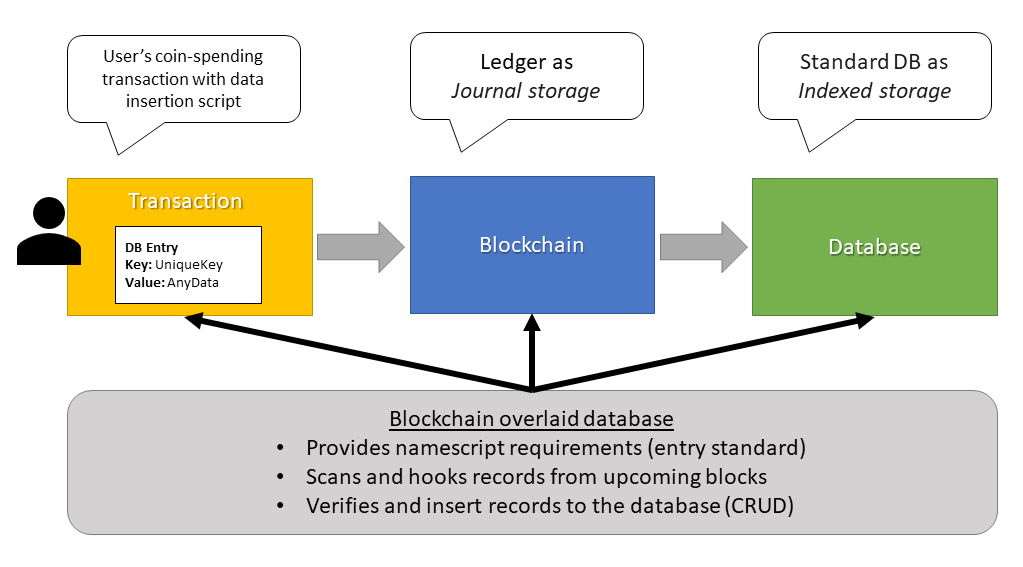
\includegraphics[scale=1.15]{src/Figures/chap1/chap1-fig02.jpg}
%~ \caption{Relation of blockchain data to key-value database}\label{chap1-fig02}
%~ \end{figure}

\begin{quote}
The system scans upcoming blocks according to the provided format standard and adds records to the database table. The entry may also contain the field which specifies till which block the entry is valid and some other data.
\end{quote}

In the first generation of DLTs (Bitcoin and similar), users apply specific scripts and methods to add arbitrary data in a coin transaction (from a few bytes up to around 100 kB per transaction including the transaction itself, i.e., in Bitcoin \cite{art1-key28}). As a result of such transaction, the coin itself is “burnt.”

In the second generation of DLTs, data insertion may have larger limits or no theoretical limits at all and are constrained by fees the user must pay for the message size. In Ethereum, for example, data insertion is performed by deploying a smart contract, which is designed as an application to store user’s arbitrary data. The combination of different types of ledgers in one bundle may require distinguishing common features and approaches, which will be reflected in the data format requirements.

\textbf{Data format.} To insert data, compliant with the cross-blockchain protocol, it must be structured in the following elements:
\begin{itemize}
\item \textit{“Key”} is a short string that identifies the user’s data; it must be unique across the bundle of blockchains. It is a searchable key in the database. In some systems it is also called “Name.”
\item \textit{“Value”} is any arbitrary data related to Key (Name).
\item \textit{“Lease time”} is a record which points out the number of a block, till the user’s key-value record will be valid. The outdated record will be erased from the database after this block. The initial record itself will be irrevocably stored in the blockchain where it has been published. This element is optional. But the developer should consider the constantly growing size of the database and can set up some defaults.
\end{itemize}

A key-value entry, or particularly an NVS record (as it is referred to Name-Value Storage technology), is attached to a user’s address in the result of a blockchain transaction, so this ensures the ownership of a record. Only the holder of the private key of the address may update or transfer the record; nobody else can publish the record with the same name while it is valid.

\textbf{Basic transactions.} There are three types of transactions: 

\begin{itemize}
\item \textbf{name new} – the creation of a new key-value record; before publishing, the record is checked with the database against its uniqueness; if the key already exists, the user may not publish it; though if the user did previously create it (the owner of the record), it can be updated;
\item \textbf{name update}, which includes
\begin{itemize}
\item[-] \textbf{value update} - the owner of the key can publish the same key, and add a new data in the field “Value;”
\item[-] \textbf{change Lease time} (reduce or extend); and 
\item[-] \textbf{transfer} key-value record to another address, and so transfer the ownership over this record; all these types of updates may be performed in the same transaction;
\end{itemize}
\item \textbf{name delete}-the owner publishes the name record with the instruction for deletion; from the block where it has been published, the records become invalid. The protocol passes the command to the database to erase the record. From the following block, any user may publish the same key again (because nobody owns it anymore).
\end{itemize}

The concept of a database across a bundle of blockchains is presented in Fig.~\ref{chap1-fig03}. The example of NVS in action is the following. The user publishes the key “Alice” and Value “+61414739692” to store the record of her public contact unless “Alice” already belongs to someone in the database. Anyone who enquires in their cross-blockchain node “Alice” will see the telephone number which belongs to a specific cryptocurrency address.

Timestamps provide the exclusiveness of keys in the database. Blockchain is a “timestamp machine,” which ensures certainty in the chronology of facts (transactions). 

The concept of blockchain timestamping is a matter of academic interest presented in several publications \cite{art1-key29}, \cite{art1-key30}, \cite{art1-key31, \cite{art1-key32} and \cite{art1-key33}.

Thus, the Name which is published first in the bundle of blockchains appears in the cross-blockchain database, any other entries with the same keys are rejected; therefore, name squatting is impossible.

Key-value storage is a “raw material” for any sort of monetary and non-monetary tokens, overlaid digital currencies, smart contracts and decentralized applications.

%~ \begin{figure}[H]
%~ \centering
%~ 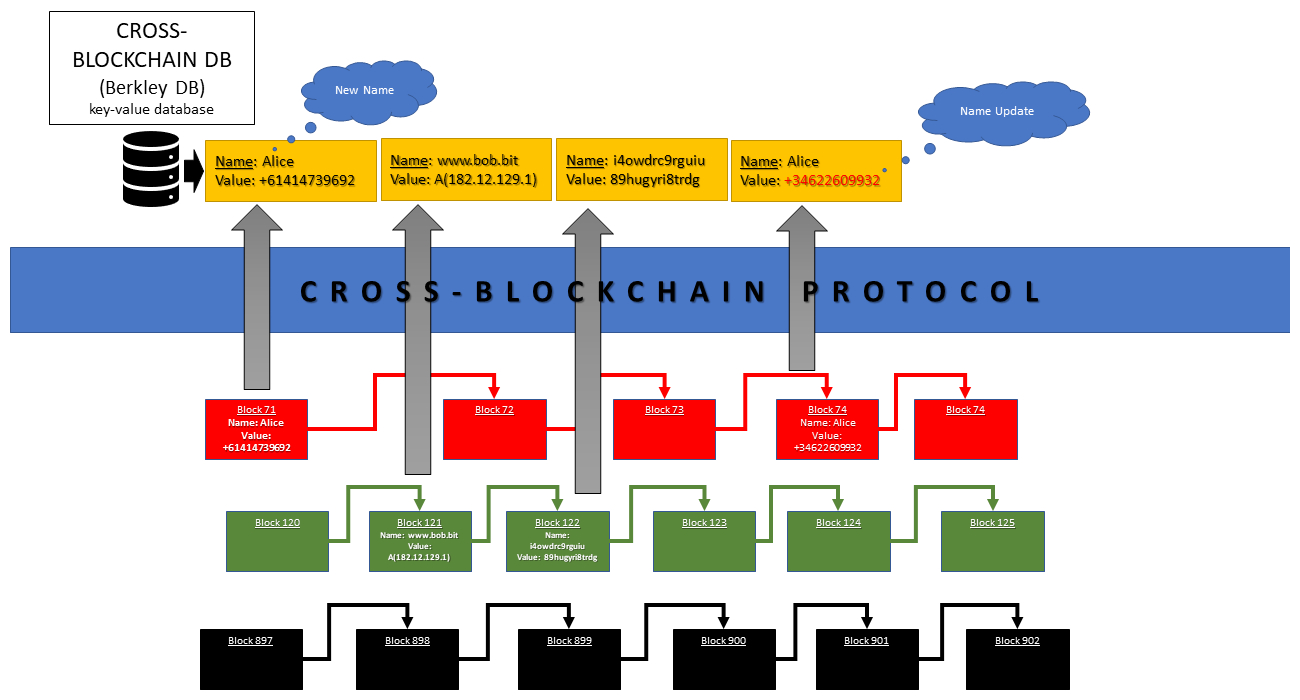
\includegraphics[scale=1.15]{src/Figures/chap1/chap1-fig03.jpg}
%~ \caption{Cross-blockchain “key-value” database}\label{chap1-fig03}
%~ \end{figure}
\begin{quote}
The scheme presents the bundle in dynamics. The system scans three ledgers: Redcoin (R), Greencoin (G), and Blackcoin (B). When it detects a complaint record, it hooks it up and adds to the overlaid database. The format is simplified; only Key and Value are traced. The hook detected blocks R-71, G-121, G-122 and R-74. Because R-74 contains the key from R-71, it updates the field Value in the relevant database record. 
\end{quote}

From the perspective of any user, a cross-blockchain database is a public storage. Every user that installed the cross-blockchain protocol and full nodes (wallets) of every blockchain of the bundle will obtain a copy of such a public database.

When the user installs the nodes, the cross-blockchain protocol hooks key-value entries from downloading blocks.

When the user enquires a key, the system retrieves the information from the user’s local storage. Besides the decentralized nature of the database, another advantage is the high speed of interaction because the copy of the database is on the local machine.

We can summarize that the cross-blockchain protocol performs two main functions, i.e., input and output.

The \textbf{“Input”} mechanism is aimed to create a key-value complaint transaction, meaning that it must contain all required fields of a new database entry. The key itself must be unique in the database and must belong to one address, and the protocol accepts it only under this condition.

The \textbf{“Output”} tool scans downloading blocks and adds hooked records to the database file and responds to users’ queries to read entries from the database.

Any updates to database records are performed through blockchain transactions. It ensures that the user will not publish a key that already exists, will not capture someone’s key, and only the owner may publish updates and transfer it.

A standard wallet with integrated key-value storage should have UI and API, which provides necessary assistance for the user to create a correct key-value transaction for the cross-blockchain database.

Nevertheless, as far as public blockchain is an uncensored system, anyone may write manually the code of the transaction, which will not be necessarily compliant and send it directly to the mempool omitting the protocol. Therefore, a non-compliant entry will not appear as the record in the database. This is the major role of the output tool – to build a database as per the rules.

\subsection{Setting and Operation of the System}\label{subsec-4.2}

\subsubsection{How and which blockchain is to include in the bundle?}\label{subsubsec-4.2.1}

The cross-blockchain protocol is based on a social consensus, the same as any blockchain protocol at a higher level, is a social consensus: the one who agrees with rules provided by the blockchain protocol installs the node and run it.

In the architecture of a future cross-blockchain database, the first step is to define which blockchains are scanned, in other words, added in the bundle, and how to add and exclude blockchains. Typically, the user will download and install the same software, assuming that in this way the user expresses the consent.

At the same time, any other designed protocol may create an entirely different database using other lists of blockchains or the same blockchains but with other rules and filters.

It is also assumed that the provider of a rightful version of the national cross-blockchain protocol may be a government and therefore, it can be centralized to some extent. Furthermore, every user may decide to use multiple versions of protocols, including those provided by the government and or any other community.

\end{multicols}








